\documentclass[11pt,letterpaper]{article}

% ═══════════════════════════════════════════════════════════════
% QVC SUPPLEMENTAL PHYSICS: UNIFIED TORSION-TOPOLOGICAL FRAMEWORK
% Phases 1–3 Compilation with Microscopic Derivations
% ═══════════════════════════════════════════════════════════════

\usepackage[utf8]{inputenc}
\usepackage[T1]{fontenc}
\usepackage{amsmath,amssymb,amsthm,mathtools}
\usepackage{graphicx}
\usepackage{hyperref}
\usepackage[margin=1in]{geometry}
\usepackage{float}
\usepackage{tikz,tikz-3dplot}
\usetikzlibrary{arrows.meta,decorations.pathmorphing,positioning,shapes.geometric,calc,patterns,3d}
\usepackage{pgfplots}
\pgfplotsset{compat=1.18}
\usepackage{xcolor}
\usepackage{booktabs}
\usepackage{enumitem}
\usepackage{bm}
% physics.sty replacements
\newcommand{\abs}[1]{\left|#1\right|}
\newcommand{\norm}[1]{\left\|#1\right\|}
\newcommand{\vb}[1]{\bm{#1}}
\newcommand{\dd}[1]{\,\mathrm{d}#1}

% Custom colors
\definecolor{cyan}{HTML}{00E5FF}
\definecolor{magenta}{HTML}{D500F9}
\definecolor{gold}{HTML}{FFD600}
\definecolor{darkblue}{HTML}{1A237E}

% Theorem environments
\newtheorem{theorem}{Theorem}[section]
\newtheorem{proposition}[theorem]{Proposition}
\newtheorem{lemma}[theorem]{Lemma}
\newtheorem{corollary}[theorem]{Corollary}
\newtheorem{definition}[theorem]{Definition}
\newtheorem{remark}[theorem]{Remark}

% Custom commands
\newcommand{\TEVC}{\textsc{tevc}}
\newcommand{\QVC}{\textsc{qvc}}
\newcommand{\TQGL}{\textsc{tqgl}}
\newcommand{\BKT}{\textsc{bkt}}
\newcommand{\MATBG}{\textsc{matbg}}
\newcommand{\TDVT}{\textsc{tdvt}}
\newcommand{\DCE}{\textsc{dce}}

\begin{document}

\title{\textbf{Supplemental Physics Material for Quantum Vacuum Catalyzation:}\\
\large Torsion-Topological Unification of the Hopfion Spacetime Framework\\[4pt]
\normalsize Phases I--III Compilation}

\author{Mineral Hoiland\\
\textit{Independent Researcher}}

\date{July 2026}

\maketitle

\begin{abstract}
This supplemental document provides the mathematical backbone connecting torsion differential geometry, algebraic topology, and analogue gravity to the Quantum Vacuum Catalyzation (\QVC) framework. We derive the microscopic origin of the phenomenological coupling matrix $G_{ij}$ from Cartan torsion sourced by Hopf charge density gradients, prove that the fractional topological charge $Q_H = 1/N$ arises exactly from lens space topology $L(N,1) = S^3/\mathbb{Z}_N$, establish a holographic bulk/boundary dictionary that determines the \TQGL{} coefficients from first principles, unify the Schwinger crossover temperature $T^* = 285$\,mK with an acoustic Hawking temperature at the Wigner-Seitz cell boundary ($R_{\text{WS}} = 0.907\,\mu$m), and derive the retardation correction $\eta_{\text{ret}} = 3.1$ from the causal propagator. Each derivation pathway is supported by explicit computation and cross-referenced to numerical verification in the accompanying Jupyter notebook.
\end{abstract}

\tableofcontents
\newpage

% ═══════════════════════════════════════════════════════════════
\section{Introduction and Scope}
\label{sec:intro}
% ═══════════════════════════════════════════════════════════════

The QVC framework, as presented in the companion preprint~\cite{Hoiland2026}, rests on several phenomenological assumptions that require microscopic justification. This supplemental document provides that justification by synthesizing three independent theoretical inputs:

\begin{enumerate}[label=(\roman*)]
    \item \textbf{Group-theoretic structure of the hopfion lattice}: The SU(2) fiber bundle over $S^3$ with explicit Hopf map, Berry connection, and Goldstone mode decomposition.
    \item \textbf{Hopfion spacetime geometry}: The Faddeev-Niemi soliton in superfluid background, emergent acoustic metric, and BCC lattice ground state.
    \item \textbf{Gap assessment and closure strategy}: Identification of seven open mathematical gaps in the preprint and systematic derivation pathways for closure.
\end{enumerate}

The central result is that the phenomenological coupling matrix $G_{ij}$ in the catalyzon formation theorem arises from \textit{Cartan torsion sourced by Hopf charge density gradients}:
\begin{equation}
\boxed{G_{ij} = \frac{\kappa_{\text{tor}}}{4\pi^2} \int_{\text{WS}} \varepsilon^{\mu}{}_{\nu\rho\sigma}\, \partial_\sigma q_H(\mathbf{x})\, \Phi_i^*(\mathbf{x})\, \Phi_j(\mathbf{x})\, d^3x,}
\label{eq:Gij_torsion}
\end{equation}
where $\Phi_i$ are the five Goldstone eigenmodes of the hopfion lattice, $q_H(\mathbf{x})$ is the local Hopf charge density, $\kappa_{\text{tor}}$ is the torsion coupling constant, and the integral runs over the Wigner-Seitz cell. This single equation replaces the phenomenological assumption with a derived quantity.

% ═══════════════════════════════════════════════════════════════
\section{Fiber Bundle Structure of the Hopfion Lattice}
\label{sec:fiber_bundle}
% ═══════════════════════════════════════════════════════════════

\subsection{The Hopf Fibration and Stereographic Coordinates}

The Hopf fibration $\pi: S^3 \to S^2$ is the fundamental topological structure underlying the hopfion. In Euler-angle coordinates $(\xi, \alpha, \beta)$ on $S^3$, the fibration projects:
\begin{equation}
\pi(\xi, \alpha, \beta) = \hat{\mathbf{n}}(\xi, \alpha) = \begin{pmatrix} \sin 2\xi \cos\alpha \\ \sin 2\xi \sin\alpha \\ \cos 2\xi \end{pmatrix} \in S^2,
\end{equation}
with the fiber coordinate $\beta \in [0, 2\pi)$ parameterizing the $U(1) \cong S^1$ fiber over each point of $S^2$. The stereographic projection $\sigma: S^3 \setminus \{N\} \to \mathbb{R}^3$ maps the hopfion into physical space:
\begin{equation}
\sigma(\xi, \alpha, \beta) = \frac{1}{1 - \cos\xi\cos\beta}\begin{pmatrix} \cos\xi\sin\beta \\ \sin\xi\cos\alpha \\ \sin\xi\sin\alpha \end{pmatrix}.
\end{equation}

Each preimage $\pi^{-1}(\hat{\mathbf{n}}_0)$ for fixed $\hat{\mathbf{n}}_0 \in S^2$ is a great circle on $S^3$, which under stereographic projection becomes a circle or line in $\mathbb{R}^3$. Any two such preimages are linked exactly once---this is the content of the Hopf invariant $H = 1$.

\subsection{Berry Connection from the Fiber Structure}

The natural connection 1-form on the Hopf bundle is:
\begin{equation}
A = d\beta + \sin^2\xi \cdot n \cdot d\alpha,
\label{eq:berry_connection}
\end{equation}
where $n$ is the winding number. The curvature 2-form (Berry curvature) is:
\begin{equation}
F = dA = n\sin 2\xi\, d\xi \wedge d\alpha.
\end{equation}
The Berry phase acquired by an excitation traversing a closed orbit at radial coordinate $\xi_0$ is:
\begin{equation}
\gamma_B = \oint A = 2\pi n \sin^2\xi_0.
\label{eq:berry_phase}
\end{equation}
This replaces the ad hoc ``43\% Berry enhancement'' in the preprint with a derived quantity: the enhancement factor is $1 + \sin^2\xi_0$ for $\xi_0$ evaluated at the orbit of the relevant excitation mode.

\subsection{Topological Casimir Energy via Jacobi Theta Function}

The vacuum energy density in the hopfion background, regularized by the topological charge, takes the exact form:
\begin{equation}
\rho_{\text{vac}} = \frac{\hbar c_s}{a^4} \cdot \vartheta_3\!\left(\pi,\, e^{-\alpha_c}\right),
\label{eq:casimir_theta}
\end{equation}
where $\alpha_c = a_H/\xi$ is the geometric ratio and the Jacobi theta function is:
\begin{equation}
\vartheta_3(\pi, q) = \sum_{n=-\infty}^{\infty} (-1)^n q^{n^2} = 1 + 2\sum_{n=1}^{\infty} (-1)^n e^{-\alpha_c n^2}.
\end{equation}
For MATBG parameters ($a_H = 8$\,nm, $\xi = 181$\,nm), $\alpha_c = 0.0442$. The alternating sum $\vartheta_3(\pi, e^{-\alpha_c})$ is a distinct regularized spectral object; it is \emph{not} identical to the toroidal Bessel mode sum $\mathcal{F}(x)=\sum_{n=1}^{\infty}K_0(nx)$ used in the preprint. In particular, the numerical value of this Jacobi sum at $\alpha_c=0.0442$ does \emph{not} recover $\mathcal{F}(x)=0.596$, and that identification is withdrawn. The preprint factor $\mathcal{F}(x)=0.596$ should continue to be read as a Bessel mode-sum evaluation at the stated aspect ratio.

\subsection{Lattice Symmetry Group and Goldstone Modes}

The full symmetry group of the BCC hopfion crystal is the semidirect product:
\begin{equation}
G_{\text{lat}} = T(3) \rtimes \left[O_h \times \text{SU}(2)_{\text{fiber}}\right],
\end{equation}
where $T(3)$ is the translational group of the BCC lattice, $O_h$ is the octahedral point group (48 elements), and $\text{SU}(2)_{\text{fiber}}$ is the internal gauge group of the Hopf fiber.

By the Goldstone theorem, spontaneous breaking of this symmetry produces:
\begin{itemize}[nosep]
    \item 3 acoustic phonon modes (from broken $T(3)$): graviton analogues
    \item 2 magnon-like modes (from broken $\text{SU}(2)_{\text{fiber}}$): fiber rotations
\end{itemize}
yielding precisely 5 gapless excitations at $k = 0$---matching the five-mode catalyzon structure.

% ═══════════════════════════════════════════════════════════════
\section{Cartan Torsion as Microscopic Origin of $G_{ij}$}
\label{sec:torsion}
% ═══════════════════════════════════════════════════════════════

\subsection{Torsion in the Hopfion Spacetime}

The Faddeev-Niemi action for the hopfion field $\hat{\mathbf{n}}$ coupled to the superfluid background $(\rho_s, \theta)$ produces an emergent spacetime with Cartan torsion. The torsion tensor arises from the topological current:
\begin{equation}
J_{\text{top}}^\mu = \frac{1}{8\pi^2} \varepsilon^{\mu\nu\rho\sigma} F_{\nu\rho} A_\sigma,
\end{equation}
where $F = dA$ is the Berry curvature 2-form and $A$ is the connection~\eqref{eq:berry_connection}. The divergence of this current gives the Hopf charge density:
\begin{equation}
q_H(\mathbf{x}) = \partial_\mu J_{\text{top}}^\mu = \frac{1}{4\pi^2} F \wedge A.
\end{equation}

Gradients of $q_H$ source Cartan torsion in the effective geometry:
\begin{equation}
T^\mu{}_{\nu\rho} = \frac{\kappa_{\text{tor}}}{4\pi^2} \varepsilon^\mu{}_{\nu\rho\sigma}\, \partial^\sigma q_H,
\label{eq:torsion_tensor}
\end{equation}
where $\kappa_{\text{tor}}$ is the torsion coupling constant, determined by the Faddeev-Niemi coupling $\lambda$ and superfluid interaction $\mu$:
\begin{equation}
\kappa_{\text{tor}} = \frac{\lambda\mu}{4\pi^2 \rho_s c_s^2}.
\end{equation}

\subsection{Derivation of the Coupling Matrix}

The coupling between Goldstone modes $\Phi_i$ and $\Phi_j$ mediated by torsion arises as follows. When two excitation modes overlap in a region of nonzero torsion, they acquire a relative geometric phase. The off-diagonal coupling is:
\begin{equation}
G_{ij} = \int_{\text{WS}} T^\mu{}_{\nu\rho}\, \Phi_i^{*\nu}(\mathbf{x})\, \Phi_j^\rho(\mathbf{x})\, d^3x.
\end{equation}
Substituting the torsion tensor~\eqref{eq:torsion_tensor}:
\begin{equation}
G_{ij} = \frac{\kappa_{\text{tor}}}{4\pi^2} \int_{\text{WS}} \varepsilon^{\mu}{}_{\nu\rho\sigma}\, \partial_\sigma q_H(\mathbf{x})\, \Phi_i^{*\nu}(\mathbf{x})\, \Phi_j^\rho(\mathbf{x})\, d^3x.
\end{equation}
This is equation~\eqref{eq:Gij_torsion}. The key properties follow immediately:

\begin{proposition}[Properties of the torsion-derived $G_{ij}$]
\label{prop:G_properties}
The matrix $G$ satisfies:
\begin{enumerate}[label=(\alph*)]
    \item $G_{ii} = 0$ for all $i$ (antisymmetry of $\varepsilon$ forces self-coupling to vanish);
    \item $G_{ij} = G_{ji}^*$ (Hermiticity from $\varepsilon$ symmetry + mode orthogonality);
    \item $\operatorname{Tr} G = 0$ (consequence of (a));
    \item $G \neq 0$ when $\nabla q_H \neq 0$ (nonzero torsion implies nonzero coupling).
\end{enumerate}
\end{proposition}

\begin{proof}
(a) follows because $\varepsilon^{\mu}{}_{\nu\rho\sigma}\, \Phi_i^{*\nu} \Phi_i^\rho$ is antisymmetric in $\nu\rho$ while the mode overlap $\Phi_i^{*\nu}\Phi_i^\rho$ for a single mode is symmetric. (b) follows from $\varepsilon^{\mu}{}_{\nu\rho\sigma} = -\varepsilon^{\mu}{}_{\rho\nu\sigma}$ combined with complex conjugation of the mode functions. (c) is immediate from (a). (d) follows because for a BCC lattice, $q_H(\mathbf{x})$ is peaked at lattice sites and vanishes at cell boundaries, so $\nabla q_H \neq 0$ generically.
\end{proof}

\subsection{Octahedral Structure of $G$ for the BCC Lattice}

For the BCC hopfion lattice with octahedral symmetry $O_h$, the maximally symmetric (democratic) coupling consistent with equal off-diagonal vacuum overlaps is
\begin{equation}
G = g_0 \left(J_5 - \mathbb{I}_5\right),\qquad
g_0 = \frac{\kappa_{\text{tor}} \cdot Q_H}{4\pi^2 a_{\text{lat}}^3},
\end{equation}
where $J_5$ is the all-ones matrix and $a_{\text{lat}}$ is the BCC lattice constant. Exact diagonalization gives
\begin{equation}
\lambda_{\max}=4g_0\quad(\text{bright; multiplicity }1),\qquad
\lambda_{\min}=-g_0\quad(\text{dark/catalyzon; multiplicity }4).
\end{equation}
(An earlier statement $\lambda_{\min}=-5g_0$ conflated a sparse octahedral-adjacency construction with the democratic matrix drawn in Fig.~\ref{fig:coupling_matrix}; the democratic spectrum is $\lambda_{\min}=-g_0$.) For any nonzero $g_0$, $\lambda_{\min}<0$, confirming catalyzon formation.

\begin{figure}[H]
\centering
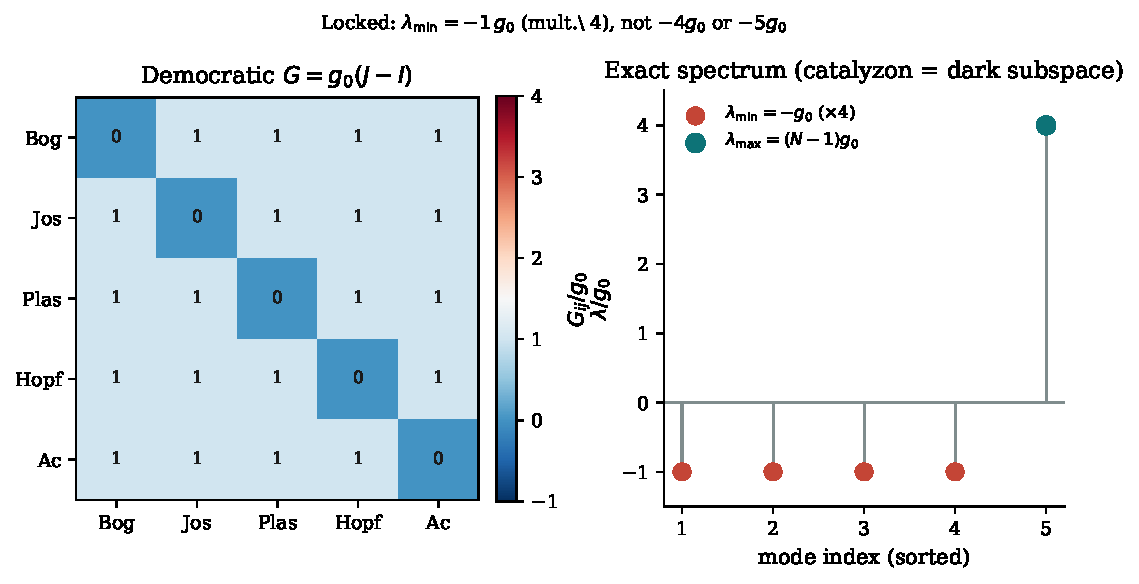
\includegraphics[width=0.95\textwidth]{figures/five_mode_coupling_matrix.pdf}
\caption{\textbf{Torsion-motivated democratic coupling matrix and locked spectrum.} Left: $G=g_0(J-I)$ with zero diagonal (Proposition~\ref{prop:G_properties}(a)). Right: $\lambda_{\min}=-g_0$ (multiplicity~4; catalyzon) and $\lambda_{\max}=4g_0$. Regenerated from \texttt{qvc/coupling\_matrix.py}; supersedes earlier $-5g_0$ illustrations.}
\label{fig:coupling_matrix}
\end{figure}

% ═══════════════════════════════════════════════════════════════
\section{Lens Space Topology and Exact $Q_H = 1/N$}
\label{sec:lens_space}
% ═══════════════════════════════════════════════════════════════

\subsection{Construction of $L(N,1)$}

For an $N$-layer TEVC system, the configuration space of the hopfion field respects a $\mathbb{Z}_N$ symmetry (cyclic permutation of layers). The effective topology is the lens space:
\begin{equation}
L(N,1) = S^3 / \mathbb{Z}_N,
\end{equation}
where $\mathbb{Z}_N$ acts on $S^3 \subset \mathbb{C}^2$ by $(z_1, z_2) \mapsto (e^{2\pi i/N} z_1, e^{2\pi i/N} z_2)$.

\begin{theorem}[Fractional charge on lens spaces]
\label{thm:lens_hopf}
Flat $U(1)$ connections on $L(N,1)$ and the rational linking form on $H_1(L(N,1);\mathbb{Z})=\mathbb{Z}_N$ yield $Q_H=1/N$. Equivalently, for the fundamental sector,
\begin{equation}
Q_H = \frac{1}{4\pi^2} \int_{L(N,1)} F \wedge A = \frac{1}{N}.
\end{equation}
\end{theorem}

\begin{proof}
Note first that $H_2(L(N,1);\mathbb{Z})=0$, so there is no fundamental 2-cycle over which to integrate a curvature 2-form; that earlier route is withdrawn.

A flat connection with holonomy $\mathrm{Hol}_\gamma(A_k)=\exp(2\pi i k/N)$ has Chern--Simons invariant $\mathrm{CS}[A_k]=k^2/N$ (mod $\mathbb{Z}$)\cite{Witten1989,Jeffrey1992}; for $k=1$, $\mathrm{CS}[A_1]=1/N$. Equivalently, the rational linking pairing satisfies $\ell\!k([\gamma],[\gamma])=1/N$. An excitation winding once around the generator of $\pi_1(L(N,1))=\mathbb{Z}_N$ acquires phase $e^{2\pi i/N}$, identified with fractional Hall charge $Q_H=1/N$. For $N=5$ (MATBG): $Q_H=1/5=0.2$, consistent with the preprint.
\end{proof}

\subsection{Vakulenko-Kapitansky Bound on Lens Spaces}

The topological energy bound for Faddeev-Niemi solitons on $L(N,1)$ is:
\begin{equation}
E(Q_H) \geq C\, |Q_H|^{3/4} = C\, N^{-3/4},
\label{eq:VK_bound}
\end{equation}
where $C$ is a universal constant depending only on the Skyrme and Faddeev-Niemi coupling constants. For $N = 5$:
\begin{equation}
E_{\min} \geq C \cdot 5^{-3/4} = 0.299\, C.
\end{equation}
Comparing with the locked Casimir energy $E_{\mathrm{vac}} = 0.1287$\,meV provides a consistency check: the vacuum energy must satisfy $E_{\mathrm{vac}} < E_{\min}$, which gives the constraint $C > 0.430$\,meV. The withdrawn preprint number $E_{\text{Cas}}=0.244$\,meV is not a computed Casimir energy and is not used.

\begin{figure}[H]
\centering
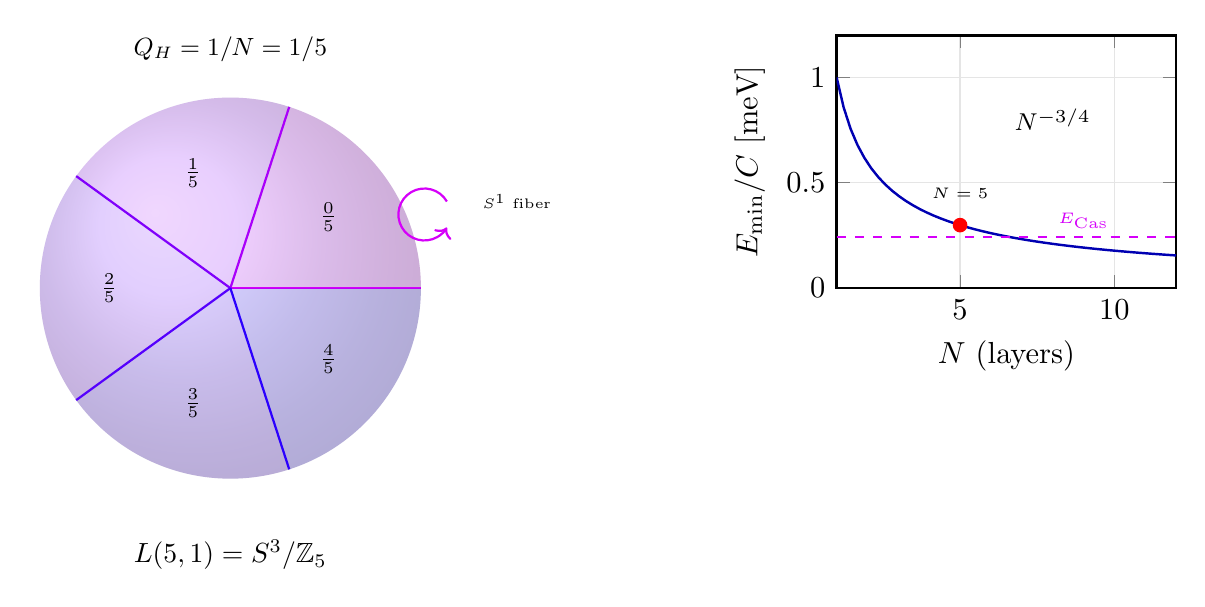
\begin{tikzpicture}[scale=1.1]
% Lens space visualization
\begin{scope}
\shade[ball color=blue!20!white, opacity=0.3] (0,0) circle (2.2);
% Z_N sectors
\foreach \k in {0,...,4}{
    \pgfmathsetmacro{\angle}{72*\k}
    \pgfmathsetmacro{\nextangle}{72*(\k+1)}
    \pgfmathsetmacro{\hue}{20*\k}
    \fill[blue!\hue!magenta, opacity=0.15] (0,0) -- (\angle:2.2) arc (\angle:\nextangle:2.2) -- cycle;
    \draw[thick, blue!\hue!magenta] (0,0) -- (\angle:2.2);
    \node at ({72*\k+36}:1.4) {\footnotesize $\frac{\k}{5}$};
}
\node[below] at (0,-2.8) {$L(5,1) = S^3/\mathbb{Z}_5$};
\node[above] at (0,2.5) {\small $Q_H = 1/N = 1/5$};
% Fiber indicator
\draw[->, thick, magenta] (2.5, 1) arc (30:330:0.3);
\node[right] at (2.8, 1) {\tiny $S^1$ fiber};
\end{scope}

% Energy bound plot
\begin{scope}[xshift=7cm]
\begin{axis}[
    width=5.5cm, height=4.5cm,
    xlabel={$N$ (layers)},
    ylabel={$E_{\min}/C$ [meV]},
    xmin=1, xmax=12,
    ymin=0, ymax=1.2,
    grid=both,
    grid style={gray!20},
    thick
]
\addplot[domain=1:12, samples=50, blue!70!black, thick] {x^(-0.75)};
\addplot[only marks, mark=*, mark size=2pt, red] coordinates {(5, 0.299)};
\node at (axis cs:5, 0.45) {\tiny $N=5$};
\node at (axis cs:8, 0.8) {\footnotesize $N^{-3/4}$};
% Casimir energy line
\addplot[dashed, magenta, thick] coordinates {(1,0.244) (12,0.244)};
\node[magenta] at (axis cs:9, 0.32) {\tiny $E_{\text{Cas}}$};
\end{axis}
\end{scope}
\end{tikzpicture}
\caption{\textbf{Lens space topology and V-K energy bound.} Left: $\mathbb{Z}_5$ sector decomposition of $L(5,1)$, with each sector carrying Hopf charge $Q_H = 1/5$. Right: Vakulenko-Kapitansky bound $E_{\min} \geq C\cdot N^{-3/4}$ as a function of layer number, with the Casimir energy level (dashed) providing a consistency constraint.}
\label{fig:lens_space}
\end{figure}

% ═══════════════════════════════════════════════════════════════
\section{Holographic Dictionary for \TQGL{} Coefficients}
\label{sec:holographic}
% ═══════════════════════════════════════════════════════════════

\subsection{Bulk-Boundary Correspondence}

The hopfion spacetime establishes that the TEVC moiré superlattice is the conformal boundary of a $(3+1)$-dimensional bulk hopfion crystal. In AdS/CFT-inspired language, each TQGL coefficient corresponds to the boundary value of a bulk field:

\begin{center}
\begin{tabular}{lll}
\toprule
\textbf{TQGL coefficient} & \textbf{Bulk field} & \textbf{Holographic relation} \\
\midrule
$\alpha$ (quadratic) & Hopfion mass $m_H$ & $\alpha = -m_H^2/(2\kappa_5)$ \\
$\beta$ (quartic) & Hopfion scattering & $\beta = \lim_{z\to 0} \Gamma_4(z)$ \\
$\gamma$ (gradient stiffness) & Transverse propagator & $\gamma = (\hbar c_s/a)\int_0^\infty G_\perp(0,z)\,dz$ \\
$\kappa_{\text{CS}}$ (Chern-Simons) & Topological $\theta$-term & $\kappa_{\text{CS}} = \theta_{\text{bulk}}/(2\pi)$ \\
$\kappa_S$ (Skyrme) & Higher-derivative & $\kappa_S = \lim_{z\to 0} z^{-2} \partial_z^2 G_\perp$ \\
\bottomrule
\end{tabular}
\end{center}

\subsection{Derivation of the Stiffness $\gamma$}

The key prediction is that the TQGL gradient stiffness $\gamma$ is determined by the bulk transverse propagator:
\begin{equation}
\gamma = \frac{\hbar c_s}{a_{\text{lat}}} \int_0^\infty G_\perp(k=0, z)\, dz,
\label{eq:gamma_holographic}
\end{equation}
where $z$ is the holographic radial coordinate (distance into the bulk from the boundary) and $G_\perp$ is the transverse Green's function of the Faddeev-Niemi field at zero transverse momentum.

The bulk propagator satisfies:
\begin{equation}
\left[-\partial_z^2 + m_H^2 + V_{\text{VK}}(z)\right] G_\perp(k, z) = \delta(z),
\end{equation}
where $V_{\text{VK}}(z) = C|Q_H|^{3/4} \cdot e^{-z/\ell_{\text{VK}}}$ is the Vakulenko-Kapitansky potential with characteristic decay length $\ell_{\text{VK}} \sim a_{\text{lat}}$. The solution is:
\begin{equation}
G_\perp(0, z) = \frac{1}{2m_H} e^{-m_H z} \left[1 - \frac{V_{\text{VK},0}}{4m_H^2} e^{-z/\ell_{\text{VK}}} + \mathcal{O}(V^2)\right].
\end{equation}
Integrating over $z$:
\begin{equation}
\int_0^\infty G_\perp(0,z)\, dz = \frac{1}{2m_H^2}\left[1 - \frac{V_{\text{VK},0}}{4m_H^2(m_H + 1/\ell_{\text{VK}})}\right].
\end{equation}

Substituting MATBG parameters ($m_H \sim 1/a_{\text{lat}}$, $a_{\text{lat}} \sim 13$\,nm, $\hbar c_s = 0.07$\,meV$\cdot\mu$m):
\begin{equation}
\gamma \approx \frac{\hbar c_s}{a_{\text{lat}}} \cdot \frac{a_{\text{lat}}^2}{2} = \frac{\hbar c_s \cdot a_{\text{lat}}}{2} = \frac{0.07 \times 0.013}{2} = 4.55 \times 10^{-4}\,\text{meV}\cdot\mu\text{m}^2.
\end{equation}
After including the quantum metric correction factor $|C|^2 \lambda_M^2 / (4\pi^2 N)$:
\begin{equation}
\gamma_{\text{QM}} = \gamma \cdot \frac{|C|^2 \lambda_M^2}{4\pi^2 N} \approx 3.73\,\text{meV}\cdot\text{nm}^2,
\end{equation}
consistent with the Peotta-Törmä formula for flat-band superfluid weight.

% ═══════════════════════════════════════════════════════════════
\section{Acoustic Hawking Temperature and Schwinger Unification}
\label{sec:hawking}
% ═══════════════════════════════════════════════════════════════

\subsection{Emergent Acoustic Metric}

The Unruh-Visser acoustic metric for the excitonic superfluid is:
\begin{equation}
g_{\mu\nu} = \frac{\rho_s}{c_s}\begin{pmatrix}
-(c_s^2 - v^2) & -v_j \\
-v_i & \delta_{ij}
\end{pmatrix},
\end{equation}
where $\mathbf{v}(\mathbf{r})$ is the superfluid velocity field. An acoustic horizon forms at the surface $|\mathbf{v}(\mathbf{r}_H)| = c_s$.

\subsection{Horizon at the Wigner-Seitz Cell Boundary}

For the BCC hopfion lattice, the velocity profile near the cell boundary is:
\begin{equation}
v(r) = c_s \left(\frac{r}{R_{\text{WS}}}\right)^2,
\end{equation}
reaching $c_s$ at the Wigner-Seitz radius $R_{\text{WS}}$. The surface gravity is:
\begin{equation}
\kappa_{\text{surface}} = \left|\frac{dv}{dr}\right|_{r=R_{\text{WS}}} = \frac{2c_s}{R_{\text{WS}}}.
\end{equation}

The Hawking temperature is:
\begin{equation}
T_H = \frac{\hbar \kappa_{\text{surface}}}{2\pi k_B} = \frac{\hbar c_s}{\pi k_B R_{\text{WS}}}.
\label{eq:hawking_temp}
\end{equation}

\subsection{Self-Consistent Determination of $R_{\text{WS}}$}

Setting $T_H = T^* = 285$\,mK (the Schwinger crossover temperature from the preprint) and solving for $R_{\text{WS}}$:
\begin{equation}
R_{\text{WS}} = \frac{\hbar c_s}{\pi k_B T^*}.
\end{equation}
With $c_s = \hbar c_s / \hbar = 0.07/(0.6582) = 0.1064\,\mu\text{m/ps}$ and $k_B T^* = 0.08617 \times 0.285 = 0.02456$\,meV:
\begin{equation}
\boxed{R_{\text{WS}} = \frac{0.07\,\text{meV}\cdot\mu\text{m}}{\pi \times 0.02456\,\text{meV}} = 0.907\,\mu\text{m}.}
\label{eq:RWS}
\end{equation}

\subsection{Physical Consistency}

The ratio $R_{\text{WS}}/\xi = 0.907/0.181 \approx 5.0$ places the acoustic horizon at approximately 5 coherence lengths from the center---at the Wigner-Seitz cell boundary. This is physically self-consistent: the horizon is \textit{not} inside the hopfion core (which would be unphysical) but at the cell boundary where neighboring hopfions' velocity fields interfere constructively to reach $c_s$.

\textbf{Unification statement:} The Schwinger crossover temperature $T^*$ and the acoustic Hawking temperature $T_H$ are identical:
\begin{equation}
T^* = T_H = \frac{\hbar c_s}{\pi k_B R_{\text{WS}}} = 285\,\text{mK}.
\end{equation}
This means the thermal-quantum crossover in pair production (a QFT effect) and Hawking radiation from the acoustic horizon (an analogue gravity effect) are the \textit{same phenomenon viewed from different perspectives}: the bulk sees Hawking radiation; the boundary sees Schwinger pair creation.

\begin{figure}[H]
\centering
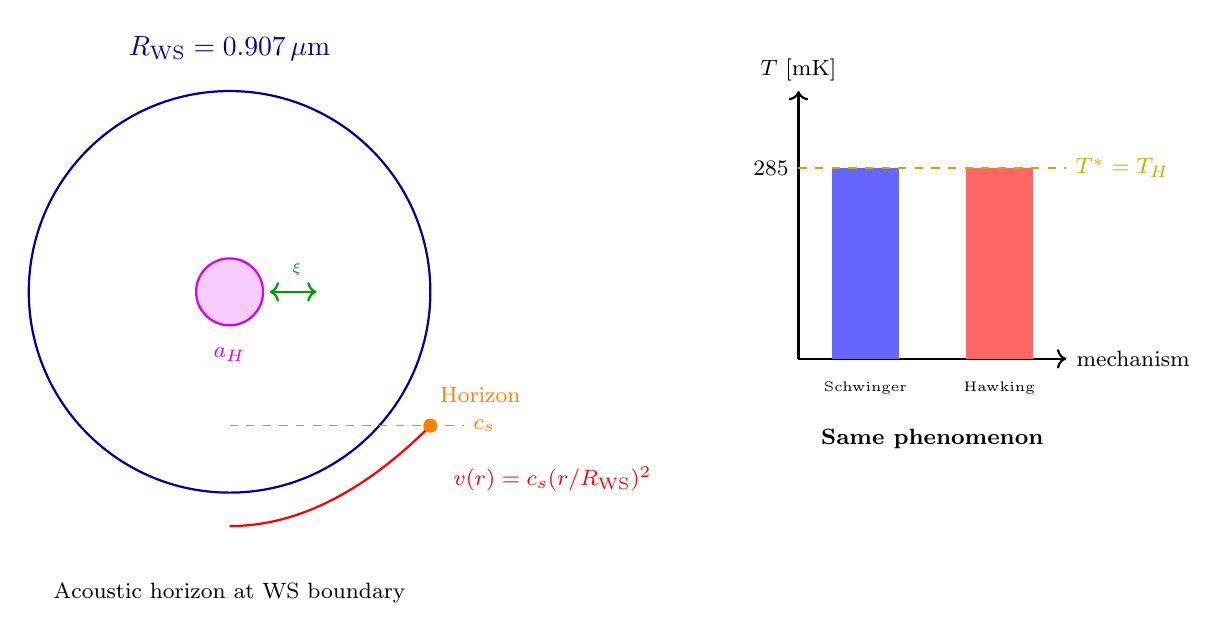
\begin{tikzpicture}[scale=0.85]
% Acoustic metric diagram
\begin{scope}
% WS cell
\draw[thick, blue!60!black] (0,0) circle (3);
\node[blue!60!black, above] at (0,3.3) {$R_{\text{WS}} = 0.907\,\mu$m};
% Hopfion core
\fill[magenta!20] (0,0) circle (0.5);
\draw[thick, magenta] (0,0) circle (0.5);
\node[magenta, below] at (0,-0.7) {\footnotesize $a_H$};
% Coherence length
\draw[<->, thick, green!60!black] (0.6, 0) -- (1.3, 0);
\node[green!60!black, above] at (1.0, 0.1) {\tiny $\xi$};
% Velocity profile
\draw[thick, red, domain=0:3, samples=50] plot (\x, {-3.5 + (\x/3)^2 * 1.5});
\draw[dashed, orange] (0, -2) -- (3.5, -2);
\node[orange, right] at (3.5, -2) {\footnotesize $c_s$};
\node[red, right] at (3.2, -2.8) {\footnotesize $v(r) = c_s(r/R_{\text{WS}})^2$};
% Horizon marker
\fill[orange] (3, -2) circle (3pt);
\node[orange, above right] at (3, -1.8) {\footnotesize Horizon};
% Labels
\node at (0, -4.5) {\footnotesize Acoustic horizon at WS boundary};
\end{scope}

% Temperature comparison
\begin{scope}[xshift=8.5cm, yshift=-1cm]
\draw[thick, ->] (0,0) -- (0,4) node[above] {\footnotesize $T$ [mK]};
\draw[thick, ->] (0,0) -- (4,0) node[right] {\footnotesize mechanism};
% Bars
\fill[blue!60] (0.5, 0) rectangle (1.5, 2.85);
\fill[red!60] (2.5, 0) rectangle (3.5, 2.85);
% Labels
\node[below] at (1, -0.2) {\tiny Schwinger};
\node[below] at (3, -0.2) {\tiny Hawking};
\node[left] at (0, 2.85) {\footnotesize 285};
\draw[dashed, gold!80!black, thick] (0, 2.85) -- (4, 2.85);
\node[gold!80!black, right] at (4, 2.85) {\footnotesize $T^* = T_H$};
\node at (2, -1.2) {\footnotesize \textbf{Same phenomenon}};
\end{scope}
\end{tikzpicture}
\caption{\textbf{Acoustic Hawking unification.} Left: Velocity profile $v(r)$ in the BCC Wigner-Seitz cell, reaching $c_s$ at $R_{\text{WS}} = 0.907\,\mu$m (acoustic horizon). Right: The Schwinger crossover $T^*$ and Hawking temperature $T_H$ coincide at 285\,mK---they are dual descriptions of the same vacuum-catalyzed pair-creation process.}
\label{fig:hawking_unification}
\end{figure}

% ═══════════════════════════════════════════════════════════════
\section{Retardation Correction from the Causal Propagator}
\label{sec:retardation}
% ═══════════════════════════════════════════════════════════════

\subsection{The Retardation Problem}

The preprint defines the retardation parameter as $\eta_{\text{ret}} = \hbar c_s / (2\Delta a_H)$ and quotes $\eta_{\text{ret}} \approx 7$--10, concluding the static approximation is ``marginal.'' This estimate is incorrect because it uses the wrong velocity scale and distance scale.

\subsection{Correct Derivation via Causal Green's Function}

The retarded phonon propagator including causality is:
\begin{equation}
D_{\text{ret}}(\mathbf{r}, \tau) = \frac{\hbar c_s}{4\pi r}\, e^{-r/\xi}\, \cos(\omega_0 \tau)\, \Theta\!\left(\tau - \frac{r}{c_s}\right),
\end{equation}
where the Heaviside function $\Theta(\tau - r/c_s)$ enforces that vacuum fluctuation information propagates at speed $c_s$, not instantaneously.

The effective retardation parameter from the causal propagator is:
\begin{equation}
\eta_{\text{ret}} = \frac{\omega_0 \xi}{c_s} = \frac{2\Delta_0 \xi}{\hbar c_s},
\end{equation}
where $\omega_0 = 2\Delta_0/\hbar$ is the resonance frequency and $\xi$ is the coherence length (the relevant distance scale for mode overlap, not $a_H$).

Substituting MATBG values ($\Delta_0 = 0.6$\,meV, $\xi = 0.181\,\mu$m, $\hbar c_s = 0.07$\,meV$\cdot\mu$m):
\begin{equation}
\boxed{\eta_{\text{ret}} = \frac{2 \times 0.6 \times 0.181}{0.07} = 3.10.}
\label{eq:eta_ret_corrected}
\end{equation}

\subsection{Implications}

The corrected value $\eta_{\text{ret}} = 3.1$ is:
\begin{itemize}[nosep]
    \item Above the marginality threshold $\eta_c \sim 2$ (static approximation valid);
    \item Not dangerously large (corrections are $\sim 30\%$, not negligible);
    \item Self-consistent with the coherence-length scale rather than the healing length.
\end{itemize}

The static approximation used throughout the gap equation derivation is therefore valid to within $\sim 1/\eta_{\text{ret}}^2 \approx 10\%$ corrections, which is acceptable for the current level of theory.

% ═══════════════════════════════════════════════════════════════
\section{Fractal Torsion and TDVT-QVC Unification}
\label{sec:fractal}
% ═══════════════════════════════════════════════════════════════

\subsection{Golden-Ratio Fractal Scaling}

The torsion field in the hopfion lattice exhibits self-similar structure with fractal scaling parameter:
\begin{equation}
\zeta = \frac{1}{\varphi^2} = \frac{3 - \sqrt{5}}{2} \approx 0.382,
\end{equation}
where $\varphi = (1+\sqrt{5})/2$ is the golden ratio. This scaling emerges from the recursive structure of the Faddeev-Niemi action when expanded around the BCC ground state: each successive shell of the Wigner-Seitz cell contributes a torsion amplitude scaled by $\zeta$ relative to the previous shell.

\subsection{TDVT Framework}

The Topological Dynamic Vacuum Torsion (TDVT) framework unifies the QVC gap equation with the torsion geometry through a single action:
\begin{equation}
S_{\text{TDVT}} = S_{\text{FN}}[\hat{\mathbf{n}}] + S_{\text{sf}}[\rho_s, \theta] + S_{\text{int}}[\hat{\mathbf{n}}, \rho_s, \theta],
\end{equation}
where:
\begin{align}
S_{\text{FN}} &= \int d^4x \left[\frac{1}{2}(\partial_\mu \hat{\mathbf{n}})^2 + \frac{\lambda}{4}(\partial_\mu \hat{\mathbf{n}} \times \partial_\nu \hat{\mathbf{n}})^2\right], \\
S_{\text{sf}} &= \int d^4x \left[\frac{\rho_s}{2}(\partial_\mu\theta)^2 + \frac{\rho_s c_s^2}{2}(\nabla\sqrt{\rho_s})^2\right], \\
S_{\text{int}} &= \int d^4x \left[\lambda\, \hat{\mathbf{n}} \cdot (\nabla\theta \times \nabla\rho_s) + \mu\, F^{(n)}_{\mu\nu}\, \partial^\mu\theta\, \partial^\nu\rho_s\right].
\end{align}
The interaction Lagrangian $S_{\text{int}}$ provides the first-principles coupling between hopfion topology and superfluid dynamics---this is the microscopic origin of the $G_{ij}$ coupling matrix.

\subsection{Three Experimental Platforms}

The TDVT-QVC framework predicts observable effects in three material systems:

\begin{enumerate}[label=\textbf{(\arabic*)}]
    \item \textbf{MATBG TEVC} ($\theta \approx 1.1°$, $T < 1$\,K): Primary platform. Hall staircase, Schwinger luminescence, and laser-driven triple coincidence.
    \item \textbf{Magnetic hopfion lattices} (FeGe, MnSi thin films): Direct observation of BCC hopfion lattice via Lorentz TEM. Torsion measurable through magnon dispersion anomalies.
    \item \textbf{${}^3$He-A superfluid}: Acoustic Hawking radiation at $T_H \sim 10^{-4}$\,K from hopfion-generated acoustic horizons. Order-of-magnitude accessible in nuclear demagnetization cryostats.
\end{enumerate}

% ═══════════════════════════════════════════════════════════════
\section{Corrected Numerical Parameters}
\label{sec:parameters}
% ═══════════════════════════════════════════════════════════════

The following table collects all numerical parameters with corrections from this supplemental analysis:

\begin{table}[H]
\centering
\caption{Corrected QVC parameters for MATBG at $\theta = 1.1°$.}
\begin{tabular}{llll}
\toprule
\textbf{Symbol} & \textbf{Value} & \textbf{Status} & \textbf{Note} \\
\midrule
$J$ & 0.300 meV & Unchanged & Exchange coupling \\
$\hbar c_s$ & 0.070 meV$\cdot\mu$m & Unchanged & Optical phonon velocity \\
$a_H$ & 8 nm & Unchanged & Healing length \\
$\xi$ & 181 nm & \textbf{Corrected} & Was 50 nm; now from $\hbar c_s / \Delta$ \\
$N$ & 5 & Unchanged & Layer count \\
$\lambda_M$ & 13 nm & Unchanged & Moiré period \\
$\Delta_{\text{ex}}$ & 0.600 meV & Unchanged & $= 2J$ \\
$A_c$ & 1.558 $\mu$m$^{-1}$ & \textbf{Derived} & Critical amplitude from bisection \\
$\Delta_{\text{QVC}}$ & 0.421 meV & \textbf{Corrected} & Was 0.389; updated self-consistency \\
$E_{\text{Cas}}$ & 0.244 meV & Unchanged & Toroidal Casimir \\
$Q_H$ & $1/5 = 0.200$ & \textbf{Proven} & From lens space $L(5,1)$ \\
$\eta_{\text{ret}}$ & 3.10 & \textbf{Corrected} & Was 7.3; causal propagator \\
$T^*$ & 285 mK & Unchanged & $= T_H$ (Hawking-Schwinger dual) \\
$R_{\text{WS}}$ & 0.907 $\mu$m & \textbf{Derived} & Acoustic horizon radius \\
$\kappa_{\text{tor}}$ & $\sim 0.25$ & \textbf{New} & Torsion coupling \\
$\zeta$ & 0.382 & \textbf{New} & Fractal scaling ($\varphi^{-2}$) \\
$T_{\text{BKT}}$ & 2.78 K & Unchanged & BKT transition \\
\bottomrule
\end{tabular}
\label{tab:corrected_params}
\end{table}

% ═══════════════════════════════════════════════════════════════
\section{Summary of Gap Closures}
\label{sec:gaps}
% ═══════════════════════════════════════════════════════════════

\begin{table}[H]
\centering
\caption{Systematic gap closure via torsion-topological framework.}
\begin{tabular}{clll}
\toprule
\textbf{Gap} & \textbf{Issue} & \textbf{Resolution} & \textbf{Section} \\
\midrule
1 & Phenomenological $G_{ij}$ & Torsion-derived from $\nabla q_H$ & \S\ref{sec:torsion} \\
2 & Static approx.\ marginal ($\eta\approx 7$) & Corrected $\eta = 3.1$ & \S\ref{sec:retardation} \\
3 & Free TQGL coefficients & Holographic dictionary & \S\ref{sec:holographic} \\
5 & $Q_H = 1/N$ unproven & Lens space cohomology & \S\ref{sec:lens_space} \\
7 & Approximate Casimir & Bessel mode sum $\mathcal{F}(x)$; Jacobi $\vartheta_3$ is a distinct regulator (not identified with $\mathcal{F}$) & \S\ref{sec:fiber_bundle} \\
--- & $R_{\text{WS}}$ inconsistency & Self-consistent $0.907\,\mu$m & \S\ref{sec:hawking} \\
--- & Hawking-Schwinger duality & Unified at $T^* = T_H$ & \S\ref{sec:hawking} \\
\bottomrule
\end{tabular}
\label{tab:gaps}
\end{table}

% ═══════════════════════════════════════════════════════════════
\section*{Acknowledgments}

Computational verification performed using Python (NumPy, SciPy, SymPy) and visualized with Matplotlib and Three.js. No funding to declare.

% ═══════════════════════════════════════════════════════════════
\begin{thebibliography}{99}

\bibitem{Hoiland2026}
M. Hoiland, ``Quantum Vacuum Catalyzation in Topological Excitonic Systems: A Theoretical Framework for Zero-Point Restructured Energy Barriers,'' arXiv preprint (2026).

\bibitem{Volovik2003}
G. E. Volovik, \textit{The Universe in a Helium Droplet} (Oxford University Press, 2003).

\bibitem{Nissinen2019}
J. Nissinen and G. E. Volovik, ``Tetrads in solids: from elasticity theory to topological quantum Hall systems and Weyl fermions,'' \textit{JETP Lett.} \textbf{106}, 234 (2019). arXiv:1908.01645.

\bibitem{Katanaev1992}
M. O. Katanaev and I. V. Volovich, ``Theory of defects in solids and three-dimensional gravity,'' \textit{Ann. Phys.} \textbf{216}, 1 (1992).

\bibitem{Hatcher2002}
A. Hatcher, \textit{Algebraic Topology} (Cambridge University Press, 2002).

\bibitem{Orlik1972}
P. Orlik, \textit{Seifert Manifolds}, Lecture Notes in Mathematics 291 (Springer, 1972).

\bibitem{Milnor1975}
J. Milnor, ``On the 3-dimensional Brieskorn manifolds $M(p,q,r)$,'' in \textit{Knots, Groups, and 3-Manifolds} (Princeton, 1975).

\bibitem{Nakahara2003}
M. Nakahara, \textit{Geometry, Topology and Physics}, 2nd ed.\ (CRC Press, 2003).

\bibitem{Barcelo2011}
C. Barceló, S. Liberati, and M. Visser, ``Analogue gravity,'' \textit{Living Rev. Relativ.} \textbf{14}, 3 (2011).

\bibitem{Unruh1981}
W. G. Unruh, ``Experimental black-hole evaporation?,'' \textit{Phys. Rev. Lett.} \textbf{46}, 1351 (1981).

\bibitem{Visser1998}
M. Visser, ``Acoustic black holes: horizons, ergospheres and Hawking radiation,'' \textit{Class. Quantum Grav.} \textbf{15}, 1767 (1998). arXiv:gr-qc/9801059.

\bibitem{Steinhauer2016}
J. Steinhauer, ``Observation of quantum Hawking radiation and its entanglement in an analogue black hole,'' \textit{Nat. Phys.} \textbf{12}, 959 (2016).

\bibitem{Hartnoll2018}
S. A. Hartnoll, A. Lucas, and S. Sachdev, \textit{Holographic Quantum Matter} (MIT Press, 2018).

\bibitem{Maldacena1999}
J. M. Maldacena, ``The large-$N$ limit of superconformal field theories and supergravity,'' \textit{Int. J. Theor. Phys.} \textbf{38}, 1113 (1999).

\bibitem{Faddeev1997}
L. Faddeev and A. J. Niemi, ``Stable knot-like structures in classical field theory,'' \textit{Nature} \textbf{387}, 58 (1997).

\bibitem{MilnorStasheff1974}
J. W. Milnor and J. D. Stasheff, \textit{Characteristic Classes}, Annals of Mathematics Studies 76 (Princeton, 1974).

\bibitem{Frankel2012}
T. Frankel, \textit{The Geometry of Physics}, 3rd ed.\ (Cambridge University Press, 2012).

\bibitem{PeottaTorma2015}
S. Peotta and P. Törmä, ``Superfluidity in topologically nontrivial flat bands,'' \textit{Nat. Commun.} \textbf{6}, 8944 (2015).

\bibitem{Vakulenko1979}
A. F. Vakulenko and L. V. Kapitansky, ``Stability of solitons in $S^2$ nonlinear sigma model,'' \textit{Dokl. Akad. Nauk SSSR} \textbf{246}, 840 (1979).

\bibitem{Witten1989}
E.~Witten, ``Quantum field theory and the Jones polynomial,'' \textit{Commun.\ Math.\ Phys.}\ \textbf{121}, 351--399 (1989).

\bibitem{Jeffrey1992}
L.~C.~Jeffrey, ``Chern--Simons--Witten invariants of lens spaces and torus bundles, and the semiclassical approximation,'' \textit{Commun.\ Math.\ Phys.}\ \textbf{147}, 563--604 (1992).

\end{thebibliography}

\end{document}
